% \documentclass{jsarticle}
% \usepackage{graphicx}
% \usepackage[dvipdfmx]{color}
% \usepackage{float}
% \usepackage{booktabs}
% \usepackage{amsmath}
% \usepackage{amsthm}
% \usepackage{array}
% \usepackage{amsmath}
% \usepackage{amsfonts}
% \usepackage[version=3]{mhchem}
% \usepackage{url}
% \usepackage{caption}
% \usepackage{here}
% \usepackage{tikz}
% \usepackage{color}
% \usepackage{url}
% \usepackage{listings,jvlisting}
% \lstset{
%   basicstyle={\ttfamily},
%   identifierstyle={\small},
%   commentstyle={\smallslshape},
%   keywordstyle={\small\bfseries},
%   ndkeywordstyle={\small},
%   stringstyle={\small\ttfamily},
%   frame={tb},
%   breaklines=true,
%   columns=[l]{fullflexible},
%   numbers=left,
%   xrightmargin=0zw,
%   xleftmargin=3zw,
%   numberstyle={\scriptsize},
%   stepnumber=1,
%   numbersep=1zw,
%   lineskip=-0.5ex
% }
% \usetikzlibrary{intersections, calc, arrows.meta}
% \usetikzlibrary{automata, positioning}
% \usepackage{algorithmic}
% \usepackage{algorithm}

%! TEX root = ../main.tex
\documentclass[../main]{subfiles}


\begin{document}
\chapter{裏磐梯に行きました} % タイトル
\rightline{M1 中原佑之助} % 学年と名前(ハンドルネームでも可)

\noindent

\section{裏合宿で裏磐梯へ行こう}
今年の天文部の正式な(?)合宿は沖縄の離島へ行くことになっていました。星も綺麗そうだし行きたかったのですが、合宿費用およそ5万円を用意することは困難でした。
そこで、2年生の惠木くんが計画してくれた裏磐梯への遠征に参加することにしました。

この記事では僕視点での裏磐梯遠征について語っていこうと思います。

\section{概要}
\subsection{日程}
2024年9月27日から29日までの二泊三日

2年前の夏合宿も全く同じような時期で懐かしさを感じました。9月末の福島は暑さが和らいできて過ごしやすい気候で良いですね。
\subsection{行き先}
行き先は、福島県は裏磐梯、曽原湖にある「湖畔のホテル クオレ」です。


聞き覚えのある人もいますかね、2022年の夏合宿、2023年の新歓合宿、2024年の新歓合宿(これには僕は行ってません)、そして今回2024年の夏遠征と、電通大天文部は何度もお世話になっています。
宿の庭から天体観測が行えること、景色が良いこと、ご飯が美味しいこと、お風呂に24時間入れること、など良いところをあげるとキリがありません。何度でも泊まりに行きたいですね。

また、今回は合宿費を抑えること、昼間の観光のしやすさ、宿からより天体観測の条件の良い場所への移動などを考えてレンタカーで移動しました。免許を持っていて運転に慣れた人が多かったこともレンタカーが利用できた要因です。


\subsection{参加者}
\begin{itemize}
\item 1年生:1人
\item 2年生:3人
\item 3年生:4人
\item 修士1年:3人
\end{itemize}
全部で11人が参加しました。天文部ではない僕の友達が3人ほどいました。主催の惠木くんから、「合宿届を出すわけではないので、誰でも参加していい」と許可がもらえたので、非天文部員も参加しています。自分の友達同士が友達になると楽しいので、僕はとても面白かったですね。新たな出会いは素晴らしいです。


\section{合宿の日記}
\subsection{1日目}
朝9時半に調布駅近くのレンタカー屋さんに集合し車に乗り込みいざ出発!


首都高に入って1時間半ほど渋滞にはまっていた気がします。オートクルーズ搭載の車だったので快適でしたが、それでも渋滞はしんどいですね。首都高を抜けると渋滞も解消され、気持ちの良いドライブができました。渋滞を抜けるとさらにオートクルーズの良さを感じました。運転していても全く疲れませんでした。

途中で那須高原サービスエリアに寄って食べたソフトクリームが美味しかったです。このサービスエリアも2年前の合宿で訪れていたので懐かしい気分になりました。


クオレに行く前に、磐梯・吾妻スカイラインという、景色の良い道をドライブしました。火山のガスや高原特有の植物などに囲まれた異国風の景色を抜け、雲と夕日を横目に登ってきた山を下りました。今までに見てきた景色の中で一番綺麗\footnote{星空を除く}と言っても過言ではないほどの絶景でした。

\begin{figure}[H]
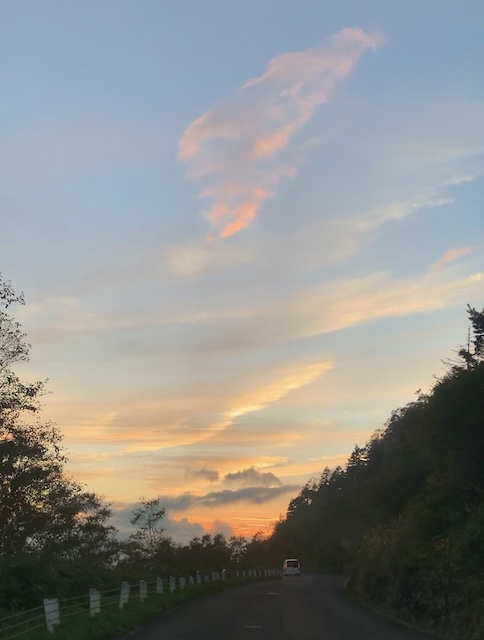
\includegraphics[width=6cm]{sections/Nakahara/IMG_8501.jpg}
\centering
\caption{ドライブ中の車窓から}
\end{figure}

ドライブを楽しんでいたら、クオレの夕食の時間に間に合わないことに気付き、電話をかけようとしましたが、標高が高いせいか電波が届きませんでした。旅にトラブルはつきものだなと思いました。結局夕食の時刻ちょうどくらいに電話をすることになりましたが、クオレさんには優しく許していただけました。その節は大変ご迷惑をおかけしました。

クオレに着くと早速夕食で、焼きそば、焼肉、お米が用意されており、夜の天体観測に備えて満腹になるまでしっかり食べました。とても美味しかったです。
\begin{figure}[H]
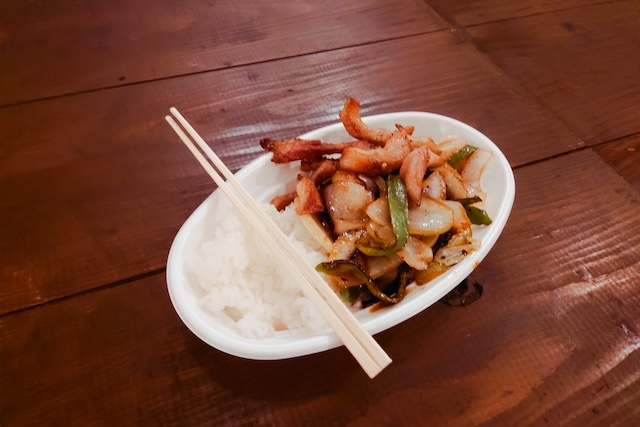
\includegraphics[width=8cm]{sections/Nakahara/IMG_8502.jpg}
\centering
\caption{1日目の夕食}
\end{figure}

クオレさんには諸事情で、電通大天文部であることを伝えていなかったのですが、3度目の訪問であること、一度会えば忘れることは難しい、オレンジ好きが高じてずっとオレンジ色のものを身につけている部員がいたことで、クオレさんには一目でバレてしまいました。「あ、そういうこと?」と全てを察していた場面は面白かったですね。

夕食を終えて風呂に入り、天体観測をはじめました。が、あいにくの天気で満足のいくほど星を見ることはできませんでした。それでも夏の天の川は肉眼でも見え、僕の大好きな冬の星空も雲の間からその姿を見せてくれました。たとえ曇っていても、都会から離れ光害の少ないところで見る満点の星\footnote{(編集部注)一般的には「満天の星」が正しい表記ですが、曇っていて``満天''ではないため、光害が少なく観測場所として``満点''という意図を汲み、この表記にしています。}はとても綺麗です。あの景色は何度見ても毎度同じように感動できます。星を見に行くことを全ての人におすすめしたいです。

初日は午前3時には眠ったと思います。僕はクオレでの朝の景色が好きなので5時半には起床し、桟橋で湖に映る磐梯山でも見ようかと思っていました。朝食の準備がされていたので、献立が気になり覗いてみると、コーヒーを入れて下さっていました。なので、桟橋の椅子に座りコーヒーを飲みながらのんびり朝を過ごしました。あのコーヒーは格別でした。

\begin{figure}[H]
\centering
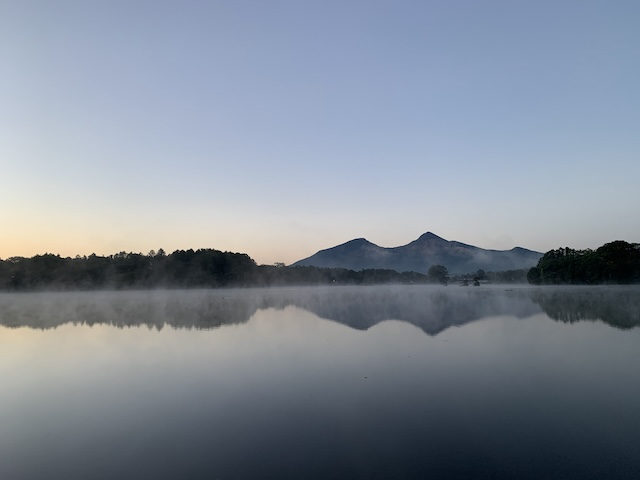
\includegraphics[width=8cm]{sections/Nakahara/IMG_2643.jpeg}
\caption{朝のクオレから見る曽原湖と磐梯山}
\centering
\end{figure}

\subsection{2日目}
2日目は福島観光組と磐梯山登山組に別れました。

1日目の夕食中に、クオレさんに2日目に磐梯山を登る予定があることを話すと、「険しくない表磐梯ルートなら幼稚園の遠足で登るレベルなので、登山靴を持っていない人も登れる」とアドバイスをいただきました。その結果、当初は修士1年3人で登山の予定でしたが、3年生の2人も参加することになりました。修士3人は険しいルート、3年生2人は表磐梯ルートで登山を楽しみました。
登山中は湖や、火山っぽい岩肌、段々と背が低くなる草木を見て楽しみました。途中温泉の匂いがしました。
頂上付近で3年生組とも合流し下山は同じルートでした。3年生の遠藤君は初めての登山でかなりしんどかったらしく、「2度と登山はしない」と誓っていました。

頂上ではしばらく景色を楽しんだり、カップラーメンを食べたり、写真を撮ったりしました。
下に広がる雲の間から山や湖が見えて綺麗でした。これまでの合宿では、磐梯山はただ眺めるだけのものだったので、登ることができてよかったです。
\begin{figure}[H]
\centering
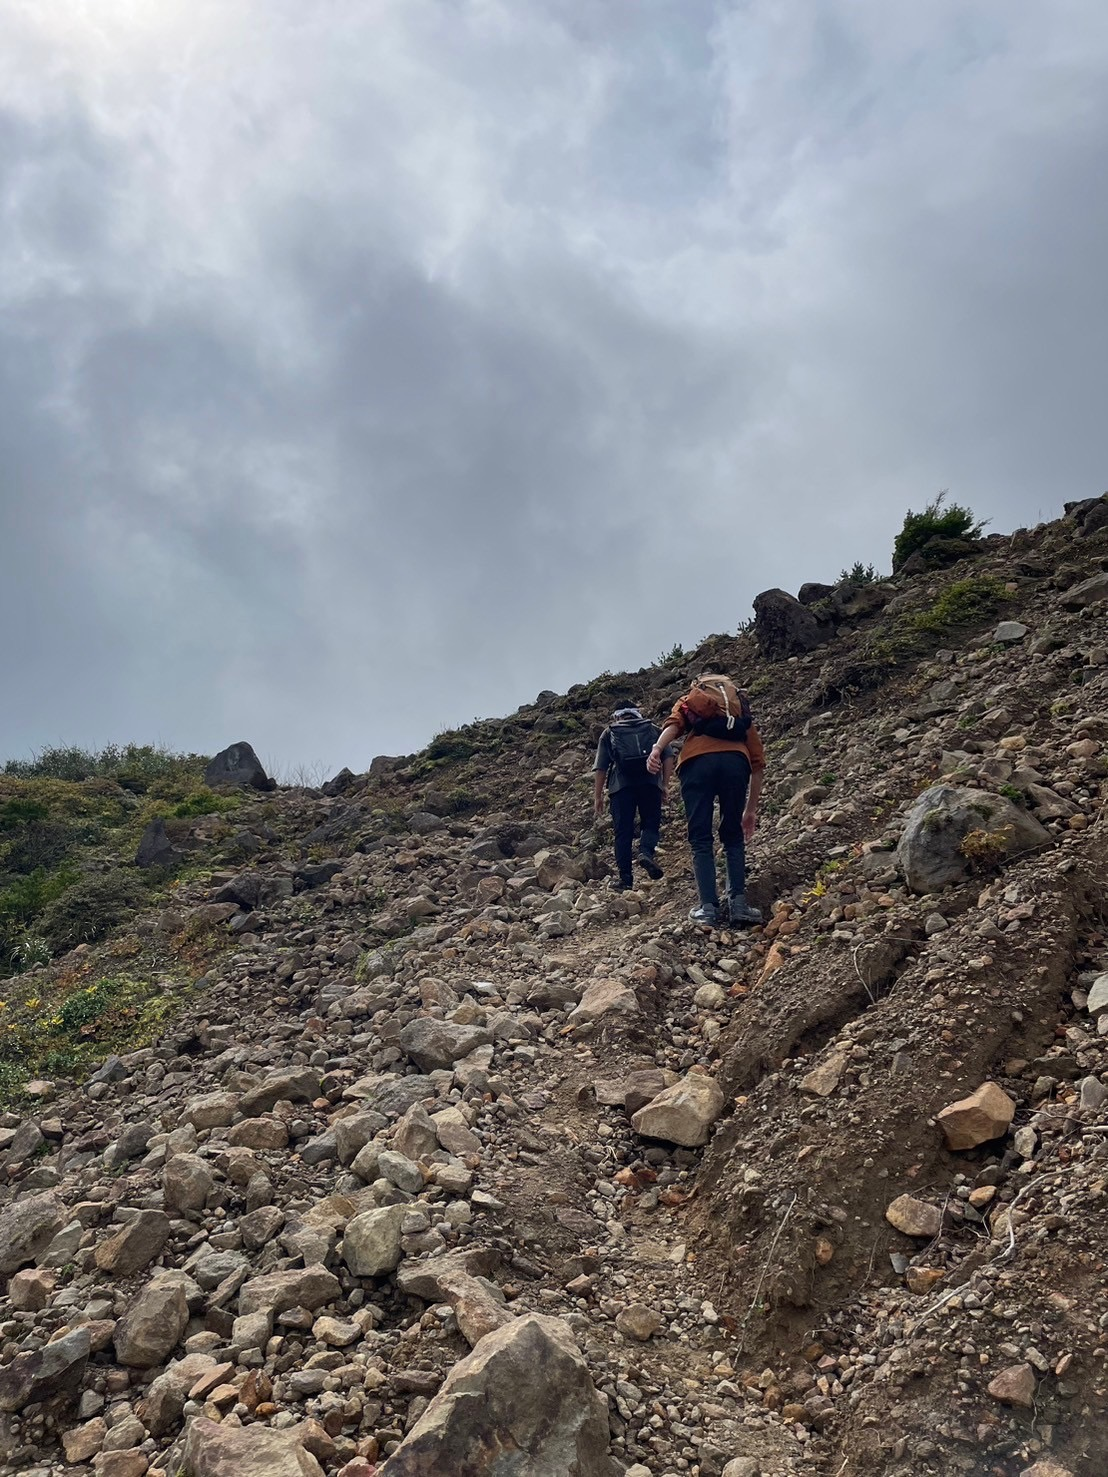
\includegraphics[width=6cm]{sections/Nakahara/IMG_8389.jpg}
\caption{登山の様子}
\centering
\end{figure}

福島観光組は、喜多方ラーメンと温泉を楽しんでいたようです。あまり詳しく聞いていませんが、みんな仲良く楽しそうだったので、良い思い出になったのではないでしょうか。

全員が宿に戻ってきて、夕食をいただき、1日目と同じように天体観測を始めました。が、またまた天気に恵まれませんでした。こればっかりは運なので仕方ないですね。曇っていると気温がそこまで下がらないので、星空を眺めながら椅子にもたれて寝ました。しばらく晴れを待ちましたが、雲はどんどんと厚みを増すばかりだったので、午前3時には部屋に戻って寝ました。

\subsection{3日目}
2日目と同じくらいに起き、またコーヒーを頂きました。この時間が一生続けばいいのになと思うくらい良い時間でした。

朝食も美味しくいただき、集合写真を撮ってもらい、ホテルを後にしました。電通大天文部であることを知らせず、得体のしれない集団だったにもかかわらずとても親切にしてくださったクオレさんには感謝してもしきれません。

帰り道の途中で、茨城のビーチに寄り少しだけ景色を楽しんだあと海鮮丼を食べました。少々値段は張りましたが美味しかったですね。僕はブリとマグロの煮切り漬け丼とマグロのユッケを食べました。
\begin{figure}[H]
\centering
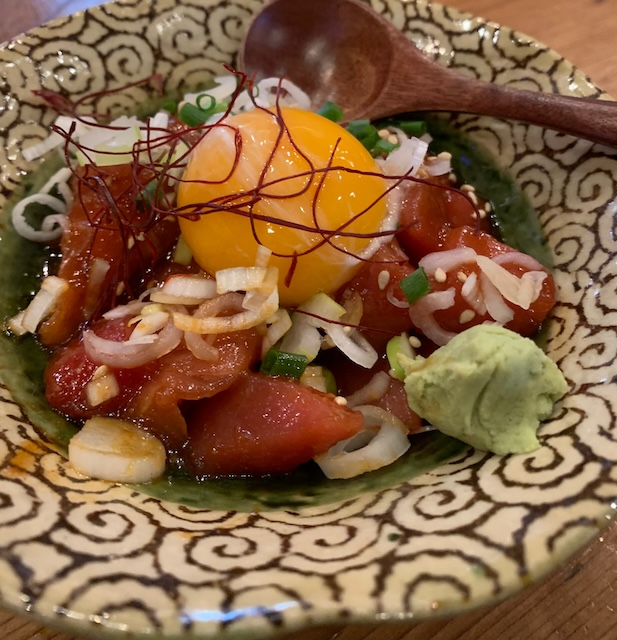
\includegraphics[width=6cm]{sections/Nakahara/yukke.jpeg}
\caption{マグロユッケ}
\centering
\end{figure}
3日目の帰路は大きな渋滞にはまることもなく、無事調布まで戻ってくることができました。事故や怪我がないのが一番ですね。

\section{まとめ}
初めてのレンタカーでの合宿でした。行動の自由度が上がるのは良いですが、翌日の運転のことを考えると天体観測で徹夜ができないのは良くないですね。今回は天気に恵まれなかったので、大人しく寝ることができましたが、快晴だったらおそらく全員がずっと起きていて、運転が不安だったと思います。一長一短ですねぇ。\footnote{個人的には、二泊三日の間寝ずに楽しんで、帰りのバスで思いっきり寝る貸切バスでの合宿が好きです。なんの心配もなく楽しめるのが最高ですね}

9月はあまり天気が良くないことと、夏の天の川が早くに沈んでしまうことを考えると来年は7月か8月に夏合宿をしたいですね。冬の星空も捨てがたいですが...。

夜の天気には恵まれませんでした\footnote{今年の天文部は天候に恵まれず新しい天体写真が少なくて調布祭に展示するものがなくて困ってる人たちがいるらしい}が、磐梯山を登り、絶景を楽しめたので個人的には良い合宿でした。
主催の惠木君や、レンタカーの手配や計画をたててくれた人たちに感謝します。またクオレに行きたいです。





\end{document}
